
\documentclass[a4paper,12pt,oneside,pdflatex,italian,final,twocolumn]{article}



\usepackage[utf8]{inputenc}
\usepackage{parallel}
\usepackage{siunitx}
\usepackage{booktabs}
\usepackage{fancyhdr}

\usepackage[export]{adjustbox}
\usepackage[margin=0.5in]{geometry}
\addtolength{\topmargin}{0in}

\usepackage{libertine}
\renewcommand*\familydefault{\sfdefault}  %% Only if the base font of the document is to be sans serif
\usepackage[T1]{fontenc}




\title{Detector de álcool SIGHIR v4.0.1}
\author{arsphotographika }
\date{April 2019}

\begin{document}

\pagestyle{fancy}

\lhead{SIGHIR}
\chead {Outubro 2024}
\rhead{Detector de álcool SIGHIR v4.0.3}


\onecolumn

\begin{figure}
\begin{minipage}{0.47\textwidth}
\centering

\includegraphics[width=.7\textwidth,left,]{logo.png}

\end{minipage}
\hfill
\begin{minipage}{0.47\textwidth}
\raggedleft
\Huge \textbf{Detector de álcool SIGHIR v4.0.2}
\end{minipage}
\end{figure}


\begin{figure}
\begin{minipage}{0.47\textwidth}

\section{Visão Geral}
    \begin{itemize}
        \item 3 modos de operação: autônomo, via bluetooth ou via comunicação serial
        \item Medições randômicas
        \item Ajustes de parâmetros via APP
        \item Calibração otimizada
    \end{itemize}


\end{minipage}
\hfill
\begin{minipage}{0.47\textwidth}
\centering
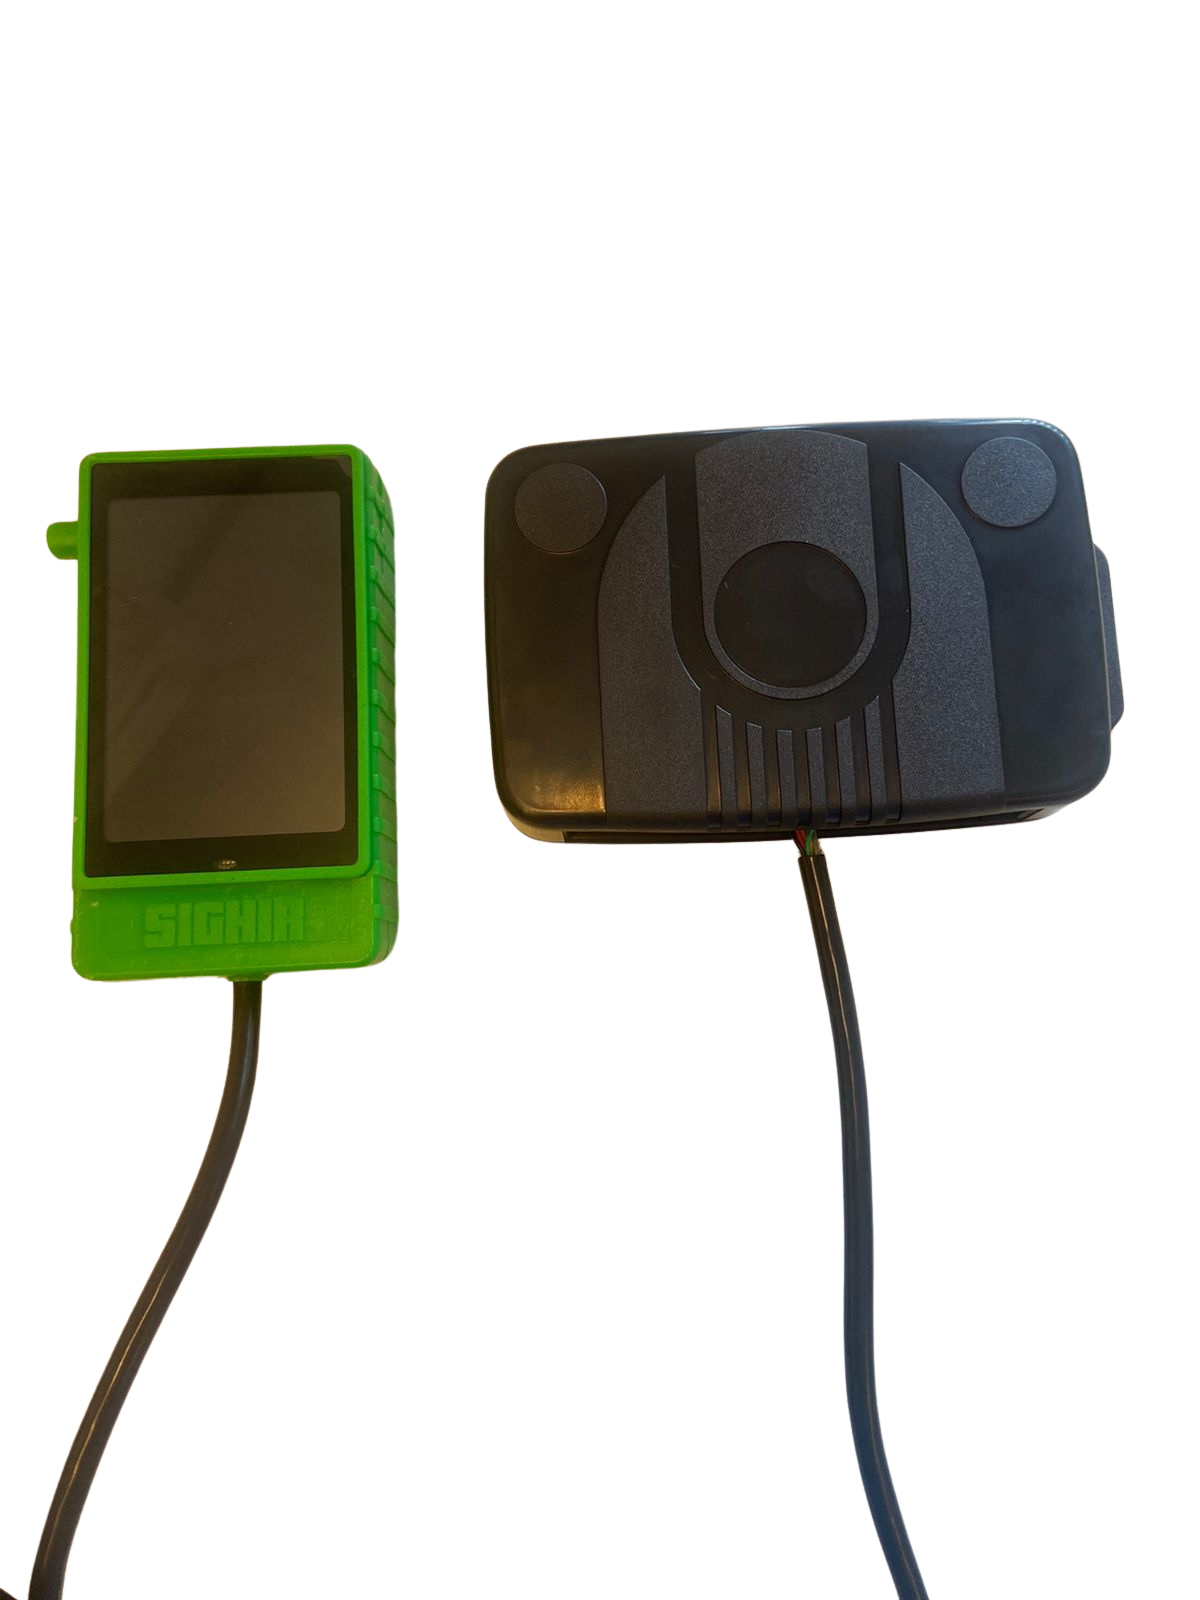
\includegraphics[width=0.7\textwidth,right]{foto.png}

\end{minipage}
\end{figure}



\section{Descrição}

A seguir, é apresentada uma breve visão geral dos recursos e especificações do dispositivo, projetado para oferecer praticidade, segurança e funcionalidade aos usuários. Confira os detalhes abaixo.

\begin{itemize}
\item Bloqueio/desbloqueio automático com base na leitura do sensor;
\item Medições aleatórias para testes durante o trajeto;
\item Ajuste de parâmetros via app móvel;
\item Atualização de firmware remota via web;
\item Autenticação com senha para desbloqueio remoto;
\item Sensor calibrado com substituição fácil pelo cliente;
\item Bocal adaptável para canudos;
\item Comunicação flexível com parceiros via serial ou Bluetooth;
\item Adiamento breve de testes quando necessário;
\item Configuração ajustável do tempo de espera de aquecimento câmera;
\item Monitoramento contínuo da temperatura.
\end{itemize}

\section{Especificações técnicas}
\centering
\begin{tabular}{lcr}
\toprule
 & Unidade & Valor \\
\midrule
Alimentação & $V$ & 12 - 40 \\
Corrente Máxima & $A$ & 4.5 \\
Dimensões exposta & $mm$ x $mm$ x $mm$ & 113 x 62.7 x 28.1  \\
Dimensões embutida & $mm$ x $mm$ x $mm$ & 129.0 x 88.0 x 28.0 \\
Peso exposta & $g$ & 140 \\
Peso embutida & $g$ & 130 \\
Temperatura de operação & $°C$ & 0 - 50\\
n° de entradas & $--$ & 2 - 5 \\
Bluetooth & $--$ & Classic v4.2 \\
WiFi & $MHz$ & 2412 - 2484 \\
WiFi & $--$ & 802.11 b/g/n (802.11n até 150Mbps) \\
Precisão & mg/L & 0.03 \\
Conexão serial & $--$ & RS232 \\
Validade do sensor & $--$ & 5000 sopros ou 2 anos \\
\bottomrule
\end{tabular}

\raggedright

\section{Pinout}

\centering
\begin{tabular}{lcr}
\toprule
  Pino & Sinal \\
\midrule
1 & GND  \\
2 & -  \\
3 & RELÉ DE BLOQUEIO   \\
4 & PÓS-CHAVE  \\
5 & ALTERNADOR \\
6 & VCC  \\ 
\bottomrule
\end{tabular}

\begin{figure}[h]
\centering
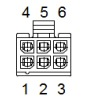
\includegraphics[width=0.2\textwidth,]{microfit.jpeg}
\end{figure}



\raggedright
\newpage
\section{Dimensões}
\centering
\begin{figure} [h]
\centering
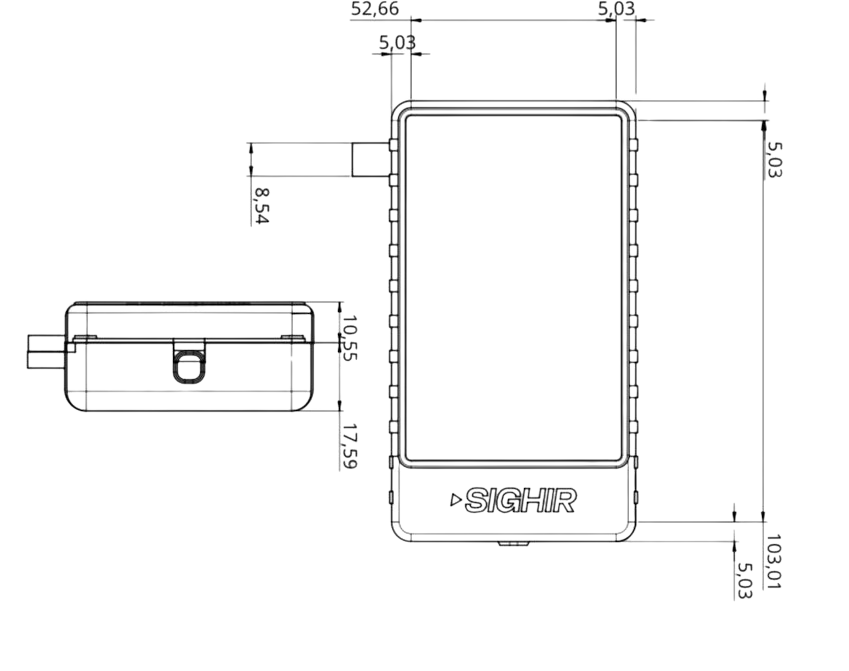
\includegraphics[width=0.5\textwidth,]{measures.png}

\end{figure}

\begin{figure} [h]
\centering
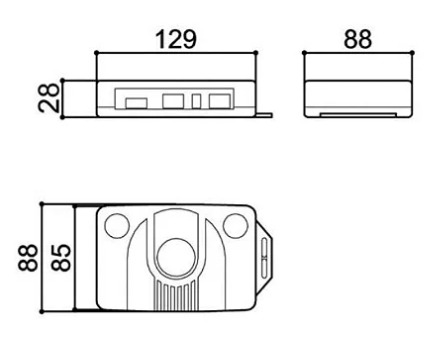
\includegraphics[width=0.5\textwidth,]{embutida.jpeg}

\end{figure}



\end{document}



